\subsection{SDMetrics}
SDMetrics is a very complete design measurement tool, analysing a wide range of UML diagrams, including Class, Usecase, Activity and Statemachine diagrams.
For each type of diagram, this tool generates several metrics.\\
For example, \textbf{NumAttr} metric, one of the metrics that has already been adressed in this paper, is calculated from Class diagrams.
Other one is \textbf{ExtPts}, wich is calculated from Usecase diagrams, and gives us the number of extension points of a given use case.\\

SDMetrics is written in java, and provides us a graphical user interface. The type of source files it receives to analyse are \textit{XMI}\footnote{
\textit{XMI} (\textbf{X}ML \textbf{M}etadata \textbf{I}nterchange)  is an \textit{OMG} (Object Management Group) standard to generate
XML-based representations of UML and other OO data models.} files, most modeling tools support project exportation in XMI.\\
This tool allows us to access the results from different views. We will approach the ones that seem the most important:
\begin{itemize}
\item \textbf{Metric Data Tables} provides a table that matches each UML model element analysed (table line) to it's value for each metric (table column);
\item \textbf{Histograms} provides a graphical distribution  for each design metric;
\item \textbf{Design Comparison} provides us a mean to compare the structural properties of two \textit{UML} designs. It is very useful to compare the same design in different iterations of the development, or to compare an alternative design to the current one.
\item \textbf{Rule Checker} design rules and heuristics detect potencial problems in the UML design such as: 
	\begin{itemize}
	\item incomplete design such as unnamed classes, states without transitions;
	\item violation of naming conventions for classes, attributes, operations, packages;
	\item etc.
	\end{itemize}
\item \textbf{Catalog} this view provides us with the definitions of the metrics, design rules, and relation matrices for the current data set, and provides literature references and a glossary for them.
\end{itemize}
Not a view, but one of the most advanced features in this software is the possibility of defining Custom Design Metrics and Rules. The new metrics are defined in a XML file, with a very particular format, the \textit{SDMetricsML} (SDMetrics Markup Language). \\
The SDMetrics tool doesn't provide a direct notion of good/bad quality of the design model. Despite that, on the SDMetrics website we can find several indications of how to interpret each kind of metrics. 
 
\subsubsection{Results}

Next we will show some printscreen's taken from SDMetrics, which will illustrate some of the outputs of this software, for our case-study.\\

\textbf{Metrics Table}
\begin{figure}[H]
\begin{center}
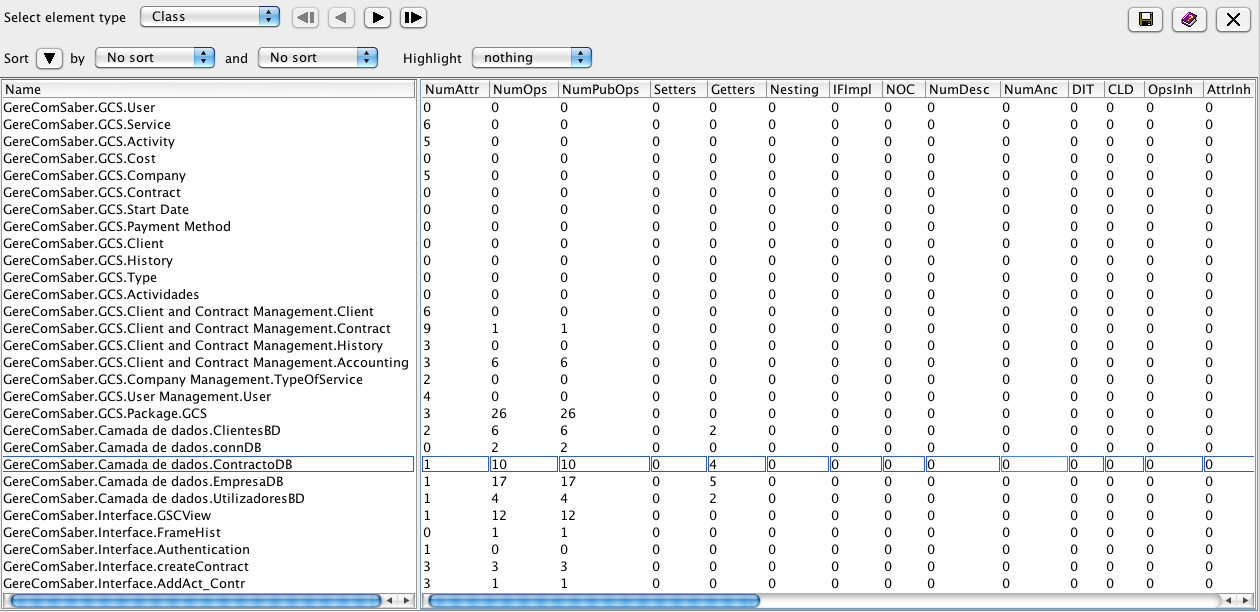
\includegraphics[width=1\textwidth]{images/table.png}
\caption{Metrics Table for class diagrams}\label{img:table}
\end{center}
\end{figure} 

\textbf{Histogram}
\begin{figure}[H]
\begin{center}
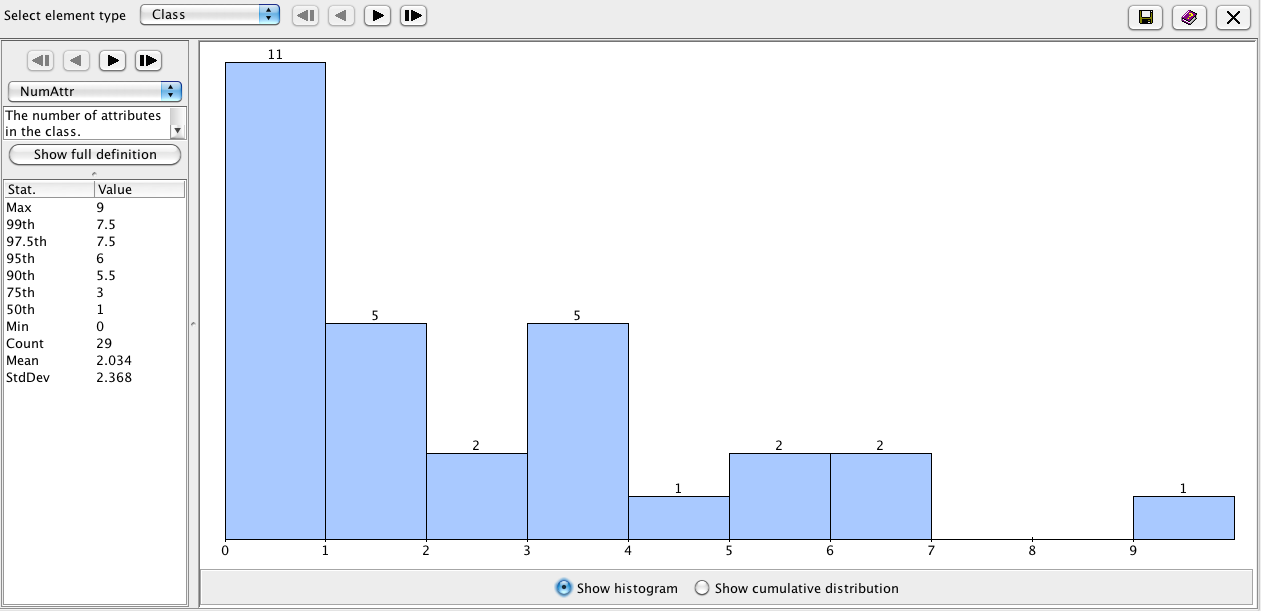
\includegraphics[width=1\textwidth]{images/histogram.png}
\caption{Histogram for class diagrams evaluating the metric NumAttr}\label{img:histogram}
\end{center}
\end{figure} 

\textbf{Rule Checker}
\begin{figure}[H]
\begin{center}
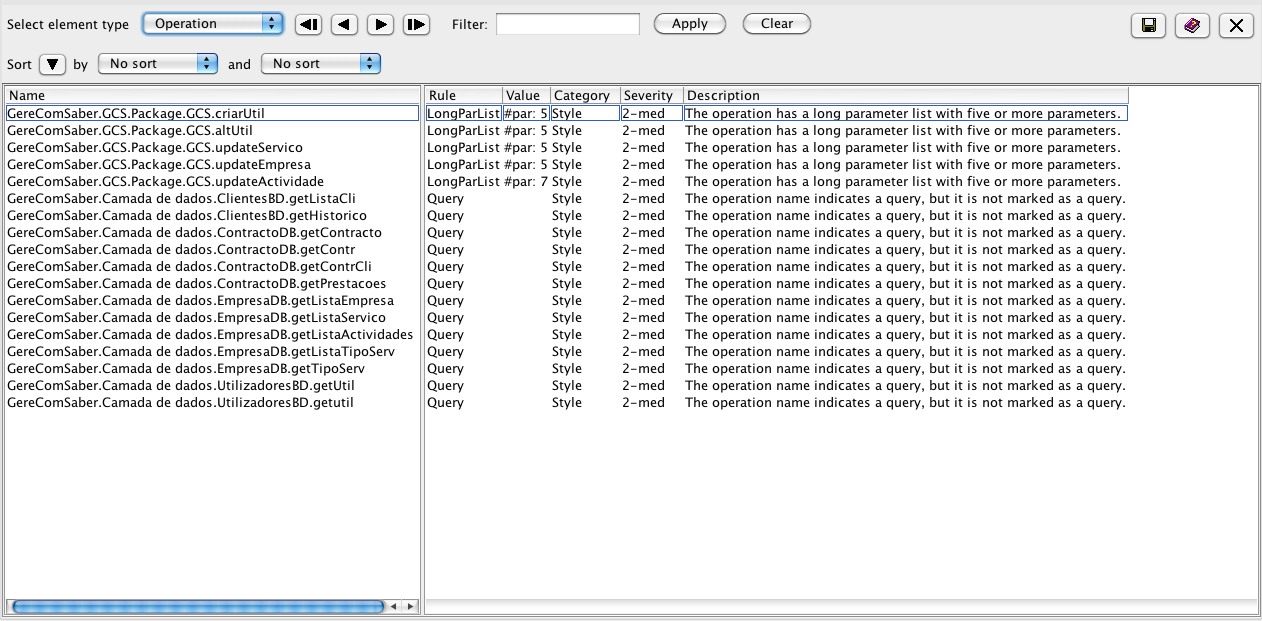
\includegraphics[width=1\textwidth]{images/rule.png}
\caption{Rule checking for Operations}\label{img:rule}
\end{center}
\end{figure} 

Based on the \textit{SDMetrics} manual, we will explain how to interpret each kind of metric, analysed by this software. \\
Size metrics, which usually count elements inside design elements (class, package, etc). The size metrics are good to estimate developing costs and effort. A large design element may indicate that it suffer's from poor design, resulting in low functional cohesion. This 	has a negative impact on the understandability, reusability, and maintainability of the design element. This size metrics can be directly found on the Metrics Table.\\
The coupling between design elements is also measured by \textit{SDMetrics}. Coupling is the degree to which the elements in a design are connected. The more the design elements are connected, the more they depend on each others. This high degree of dependency may affect the system maintainability, because when you change a design element, you may need to adapt the connected elements; and the system testability, because a problem in a design element may cause failure in a completly diferent conected element. Taking this in consideration, it is important to minimize coupling.\\
Inheritance-related metrics usually calculate features such as depth/width of the inheritance and number of ancestors/descendents of a design element. Such as high coupled elements, deep inheritance structures are believed to be more fault-prone. It is harder to fully understand a class that is situated deep in the inheritance tree, because you have to understand it's ancestor's. Also, modifying a design element with many descendants, may have a large impact on the system.\\
Complexity metrics measure the degree of connectivity between elements of a design element. They are concerned with relationships/dependencies between the elements in the design unit, such as the number of method invocations inside a class. The high complexity between the elements of a design element can make the design harder to understand, therefore more propitious to faults. Complexity metrics are usually strongly correlated with size measures. So even though they are good indicatures of quality, such as fault-proneness, they provide no new knowledge comparing to size metrics.\\
FALTA-ME FALAR DAS COHESION METRICS


 
